\documentclass[a4paper]{article}
\usepackage{graphicx} % Required for inserting images
\usepackage{wrapfig}
\usepackage{enumitem}
\usepackage[center]{caption}
\usepackage[english, russian]{babel}
\usepackage{amsmath}
\usepackage{geometry}
\geometry{verbose, a4paper, tmargin=2cm, bmargin=2cm, lmargin=2.0cm, rmargin=2.0cm}

\begin{document}

\begin{titlepage}
	\centering
	{\scshape\Large МОСКОВСКИЙ ФИЗИКО-ТЕХНИЧЕСКИЙ ИНСТИТУТ \\
	(НАЦИОНАЛЬНЫЙ ИССЛЕДОВАТЕЛЬСКИЙ УНИВЕРСИТЕТ)\\ % название ВУЗа большим шрифтом
    Физтех-школа аэрокосмических технологий}
	
	\vspace{4cm} % отступ 4 см по вертикали
	{\LARGE Отчет о выполнении лабораторной работы 1.1.1}
	
	\vspace{1cm} % ещё 1 см
	{\huge\bf Определение удельного сопротивления нихромовой проволоки}
	
	\vspace{1cm} % ещё 1 см
	\vfill % заполнение по вертикали пустотой (LaTeX сам решит, сколько здесь отступить)
	
    \begin{flushright} % Этот текст будет с правого края страницы
	   {\LARGE Ефремова Татьяна, Б03-503}
    \end{flushright}
    \vfill

	\today % Дата сборки документа
\end{titlepage}

\section{Аннотация}
Цели работы: измерить удельное сопротивление нихромовой проволоки; вычислить систематические и случайные погрешности при использовании линейки, микрометра, штангенциркуля, вольтметра, амперметра и моста постоянного тока.

\begin{wrapfigure}{R}{0.3\textwidth}
    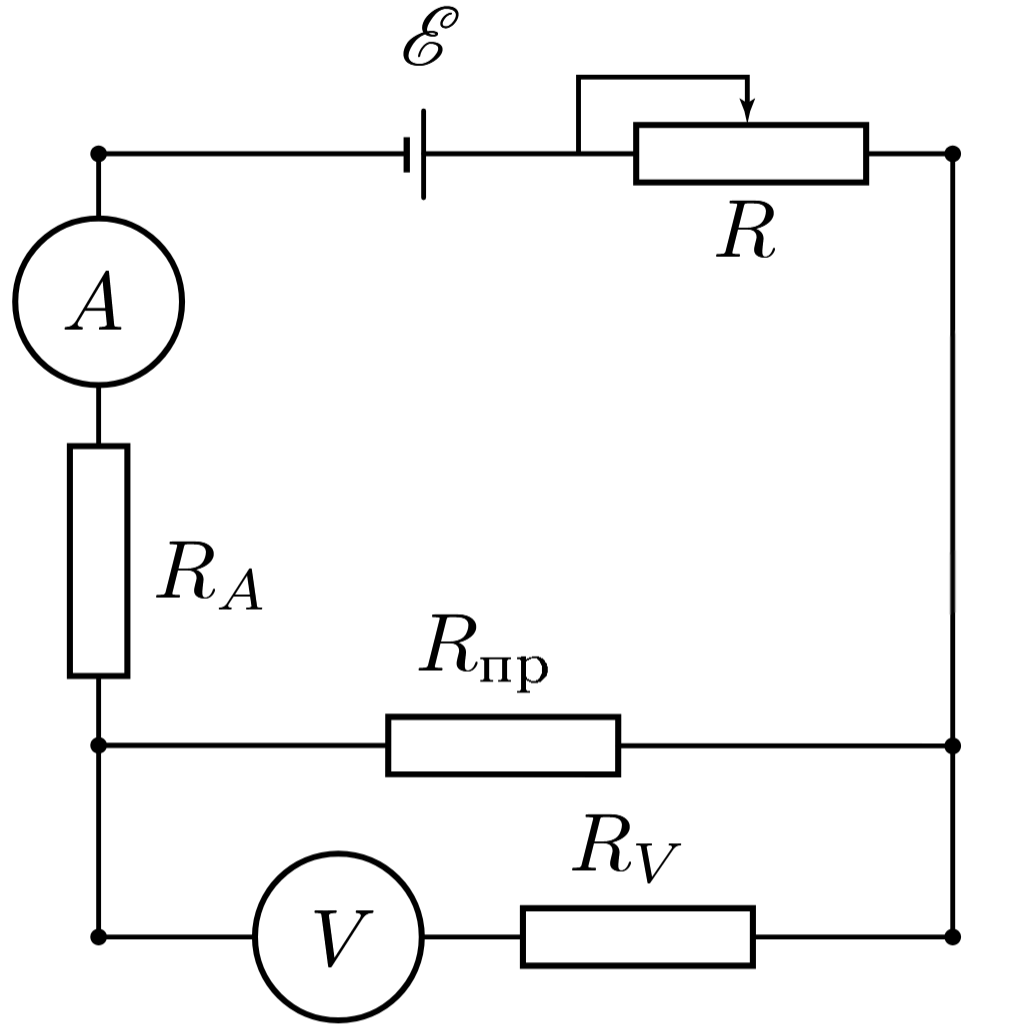
\includegraphics[width=1\linewidth]{C:/Users/User/Documents/mipt_takonef/лабы/1.1.1/1.1.1_scheme.PNG}
    \caption{Схема цепи}
\end{wrapfigure}

\section{Теоретические сведения}
Удельное сопротивление проволоки круглого сечения:
\begin{equation}
\rho = \frac{R_\text{пр}}{l}\frac{\pi d^2}{4},
\end{equation} где $R_\text{пр}$ -- сопротивление проволоки, $d$ -- диаметр, $l$ -- длина. \\
Сопротивление параллельного соединения проволоки и вольтметра:
\begin{equation}
R_\text{пр1} = \frac{V_\text{v}}{I_\text{a}},    
\end{equation}
где  $V_\text{v}$ -- напряжение вольтметра, $I_\text{A}$ -- сила тока через амперметр. \\
Ввиду неидлеальности вольтметра, спротивление проволоки:
\begin{equation}
    R_\text{пр} =\frac{R_\text{v}R_\text{пр1}}{R_\text{v}-R_\text{пр1}},
\end{equation}
где $R_\text{v}$ -- сопротивление вольтметра.

\section{Оборудование}
\subsection{Используемое оборудование}
Отрезок нихромовой проволоки, вольтметр, амперметр, источник ЭДС, мост постоянного тока, реостат, линейка, штангенциркуль, микрометр.
\subsection{Инструментальные погрешности}
\vspace{0.15 cm}

\setdescription{leftmargin=0pt}
\begin{description}
    \item[линейка:] $\Delta_\text{лин}=\pm0,5$ мм (маркировка производителя). 
    При определении положений контактов имеется дополнительная погрешность, которая может быть оценена как $\Delta_\text{лин} \approx \pm 2$ мм.
    \item[штангенциркуль:] $\Delta_\text{шт}=\pm0,1$ мм (маркировка производителя).
    \item[микрометр:] $\Delta_\text{мкм}=\pm0,01$ мм (маркировка прозиводителя).
    \item[амперметр:] абсолютная погрешность в диапазоне $80-150$ мА: $\Delta_\text{А} = \pm 0.01$ mA.

    \item[вольтметр:] шкала линейная, 150 делений; класс точности -- 0.5; предел измерений -- 0.75В. 
    \\ Абсолютная погрешность по цене деления: $\Delta_\text{В} = \pm \frac{0,75}{150*2} = \pm 2.50$ mV;
    \\ Абсолютная погрешность по классу точности: $\Delta_\text{В} =\pm \frac{0,75*0,5}{2} = \pm 1.875$ mV.

    \item[мост постоянного тока Р4833:] разрядность магазина сопротивлений -- 5 ед; класс точности -- 0,1; 
    \\ Используемый диапазон измерений: $10^{-4}$ – 10 Ом (для множителя $N = 10^{-2}$). \\
    Погрешность измерений в используемом диапазоне: $\Delta_\text{мпт} =\pm0,010$ Ом.
\end{description}

\section{Результаты измерений и обработка данных}
\subsection{Измерение диаметра $d$ проволоки}
\vspace{-0.5cm}
\begin{table}[h]
\caption{Измерения диаметра проволоки штангенциркулем и микрометром}

\centering
\begin{tabular}{|c|c|c|c|c|c|c|c|c|c|c|}
\hline
& 1 & 2 & 3 & 4 & 5 & 6 & 7 & 8 & 9 & 10\\
\hline
$d_\text{шт},$ мм & 0,4 & 0,4 & 0,4 & 0,4 & 0,4 & 0,4 & 0,4 & 0,4 & 0,4 & 0,4\\
\hline
$d_\text{мкм},$ мм & 0,36 & 0,37 & 0,36 & 0,36 & 0,37 & 0,36 & 0,35 & 0,36 & 0,36 & 0,36\\
\hline
\end{tabular}
\end{table}
\centering
$\bar{d}_\text{шт} = 0,4$ мм; $\bar{d}_\text{мкм} = 0,361$ мм

\raggedright
При измерении диаметра проволоки штангенциркулем отсутствует случайная погрешность, т.е. результат измерений определяет лишь точность прибора:
$d_\text{шт} = 0,4$ $\pm$ $0,1$ мм. \\
При измерении диаметра проволоки присутствуют как случайная, так и систематическая погрешности:

\centering
 $ \sigma_\text{отд} = \sqrt{\frac{1}{N-1} \sum_{i=1}^{N} (d_i - \bar{d})^2} \approx   6 \cdot 10^{-3} $ мм;  
$\sigma_\text{ср} = \frac{\sigma_\text{отд}}{\sqrt{N}} \approx  2 \cdot 10^{-3} $ мм; 
$ \sigma_{\text{полн}} = \sqrt{\sigma_\text{ср}^2 + \Delta_\text{мкм}^2} \approx 0,01$ мм;

\raggedright
Т. к. $ \sigma_\text{ср} <<  \sigma_\text{мкм}$, можно считать, что проволока однородная,  а погрешность при измерении ее диаметра определяется лишь точностью микрометра: 
$d_\text{мкм} = 0,361$ $\pm$ $0,010$ мм. \\

\subsection{Измерение сопротивления $R_\text{пр}$ проволоки}

Результаты измерений зависимостей показаний вольтметра $V$ от показаний амперметра $I$ в
схеме рис. 1 при разных длинах $l$ проволоки представлены в табл. 2. Соответствующие графики
зависимостей изображены на рис. 2.

\begin{table}[h]
\setlength{\tabcolsep}{0.15cm}
\renewcommand{\arraystretch}{1.6} 
\caption{Показания приборов и значения сопротивления}
\centering
\begin{tabular}{|c|c|c|c|c|c|c|c|c|c|c|c|c|c|c|}
\hline
\multicolumn{15}{|c|}{ $l = 50$ см} \\
\hline
$I,$ mA  & 30,5 & 40,6 & 50,7 & 60,7 & 75,2 & 81,0 & 85,7 & 90,8 & 99,9 & 110,8 & 120,5 & 131,0 & 140,0 & 150,3 \\
\hline
$U,$ mV & 150 & 200 & 250 & 300 & 375 & 402 & 425 & 450 & 500 & 550 & 600 & 650& 700 & 750 \\
\hline
$R$, Ом & 4,918 & 4,926 & 4,931 & 4,942 & 4,986 & 4,969 & 4,959 & 4,959 & 5,001 & 4,964 & 4,979 & 4,962 & 5,0 & 4,991 \\

\hline
\multicolumn{15}{|c|}{ $l = 30$ см} \\
\hline
$I,$ mA & 35,5 & 39,3 & 52,0 & 59,9 & 69,6 & 76,3 & 85,3 & 101,4 & 110,5 & 119,6 & 148,0 & 161,6 & 205,1 & 218,7 \\
\hline
$U,$ mV & 100 & 110 & 150 & 175 & 200 & 225 & 250 & 300 & 325 & 350 & 450 & 500 & 610 & 650 \\
\hline
$R$, Ом & 2,817 & 2,799 & 2,885 & 2,922 & 2,874 & 2,949 & 2,931 & 2,959 & 2,940 & 2,926 & 3,041 & 3,094 & 2,974 & 2,972 \\

\hline
\multicolumn{15}{|c|}{ $l = 20$ см} \\
\hline
$I,$ mA & 69,9 & 86,6 & 101 & 113,3 & 137,9 & 149,9 & 161,6 & 189 & 206,2 & 222,1 & 240,0 & 297,0 & 323,0 & 350,0 \\
\hline
$U,$ mV & 140 & 175 & 200 & 225 & 275 & 300 & 325 & 375 & 415 & 450 & 490 & 595 & 655 & 710 \\
\hline
$R$, Ом & 2,003 & 2,021 & 1,980 & 1,986 & 1,994 & 2,001 & 2,011 & 1,984 & 2,013 & 2,026 & 2,042 & 2,003 & 2,028 & 2,029 \\
\hline
\end{tabular}
\end{table}

Внутреннее сопротивление вольтметра $R_B = \frac{0,75 \text{ B}}{0,135 \text{ мА}} = 5$ кОм.\\
Т.к. поправка измерения $\frac{R_\text{пр}}{R_B} = 0,1 \%$ дает изменение не более, чем $\delta R = 5 \cdot 10^{-3}$ Ом, нет смысла пересчитывать значения сопротивления. Будем работать с данными, представленными в табл. 2.

\centering
\begin{figure}[h]
   \centering    
    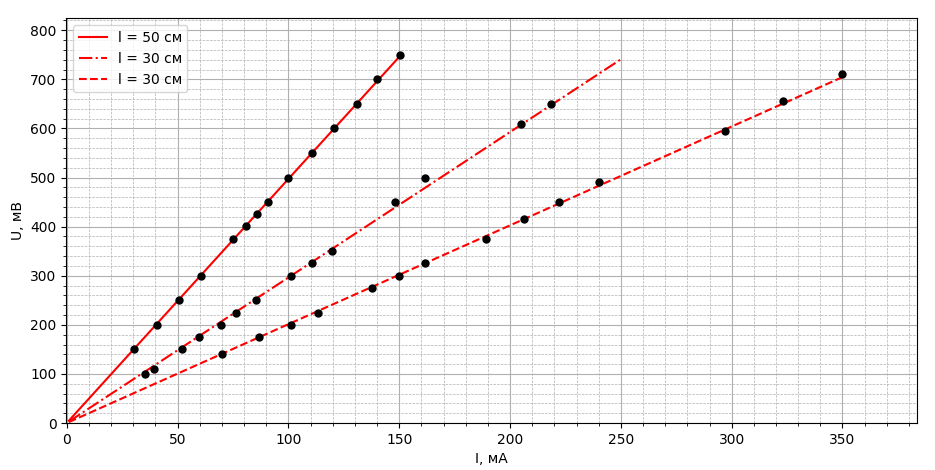
\includegraphics[width=1.01\linewidth]{C:/Users/User/Documents/mipt_takonef/лабы/1.1.1/1.1.1_plot.png}
    \caption{Линейная аппроксимация результатов измерения напряжения V \\ в зависимости от силы тока I методом наименьших квадратов} 

\end{figure}


\begin{table}[h]
\renewcommand{\arraystretch}{1.7} 
\caption{Погрешности и результаты измерения сопротивления проволоки}
\centering
\begin{tabular}{|c|c|c|c|}
\hline
& $l = 50$ см &  $l = 30$ см &   $l = 20$ см  \\
\hline
$R_0$, Ом  & 5,090 & 3,051 & 2,093 \\
\hline
$R_\text{ср} = \frac{\sum_{i=1}^{N}V \cdot I}{\sum_{i=1}^{N}I^2}$, Ом & 4,977 & 2,981 & 2,017 \\
\hline
$\sigma_\text{отд} = \sqrt{\frac{1}{N-1} \sum_{i=1}^{N} (R_i - R_\text{ср})^2} $, Ом  & 0,779  & 1,218 & 0,232 \\
\hline
$\sigma_\text{ср} = \frac{\sigma_\text{отд}}{\sqrt{N}} $, Ом  & 0,208  & 0,325 & 0,062 \\
\hline
$\sigma_\text{сист} = R_\text{ср} \sqrt{\left(\frac{\Delta_B}{V_{\text{max}}}\right)^2 + \left(\frac{\Delta_A}{I_{\text{max}}}\right)^2} $, Ом  & 0,012  & 0,008 & 0,005 \\
\hline
$\sigma_\text{полн} = \sqrt{\sigma_\text{ср}^2 + \Delta_\text{мкм}^2}$, Ом  & 0,208  & 0,325 & 0,062 \\
\hline
\end{tabular}
\end{table}
\raggedright

Итак, \\
$R_\text{$l=50$} = 4,977 \pm 0,208$ Ом, \\
$R_\text{$l=30$} = 2,981 \pm 0,325$ Ом, \\
$R_\text{$l=20$} = 2,017 \pm 0,062$ Ом. \\

\subsection{Вычисление удельного сопротивления $\rho_\text{пр}$ проволоки}

\begin{table}[h]
\renewcommand{\arraystretch}{1.7} 
\caption{Погрешности и результаты измерения сопротивления проволоки}
\centering
\begin{tabular}{|c|c|c|c|}
\hline
& $l = 50$ см &  $l = 30$ см &   $l = 20$ см  \\
\hline
$\rho = $ (1), Ом $\cdot$ м  & $1,019 \cdot 10^{-6} $ & $1,017 \cdot 10^{-6} $ & $1,032 \cdot 10^{-6} $ \\
\hline
$ \sigma_\rho = \rho\sqrt{\left( \frac{\sigma_R}{R} \right)^2 +\left( \frac{\sigma_d}{d} \right )^2 + \left( \frac{\sigma_l}{l} \right )^2} $
, Ом $\cdot$ м & 0,051 $\cdot$ $10^{-6}$ & 0,114 $\cdot$ $10^{-6}$  & 0,044 $\cdot$ $10^{-6}$ \\
\hline
\end{tabular}
\end{table}
\raggedright

$\rho = (1,022$ $\pm$ $0,070)$ $\cdot$ $10^{-6}$ Ом $\cdot$ м $(\epsilon_\rho = 6,8 \%)$

\section{Выводы}
В результате работы было измерено удельное сопротивление образца нихромовой проволоки с точностью $\approx 6,8 \%$. Табличные значения для нихрома при $20^{\circ}$ лежат в диапазоне от $1,12 \cdot 10^{-6}$ м до $0,97 \cdot 10^{-6}$ (согласно справочнику "Физические величины. М.: Энергоиздат, 1991. С. 444). Наиболее близкое значение к полученному в работе имеет сплав $70-80\%$ Ni, $ 20\%$ Cr, $0-2\%$ Mn, однако точно определить марку сплава погрешность измерений не позволяет. Для уменьшения ее требуется проиозводить измерения на более точном оборудовании, т.к. систематическая погрешность вносит в результат куда больший вклад, чем случайная, и просто увеличить количество измерений будет недостаточно.

\end{document}
